\section{永恒的陀螺}

\subsection{你是凭什么想到这个的?}

学物理最困惑我们的是,“你是凭什么想到这个的?”

如果有人能够把物理学家发现的思维过程一步一步给我们展示出来就太好了,这么做的好处,首先是欣赏,欣赏一个大师如何被一个现象吸引、困扰,进而定义问题,做出种种尝试,然后是挫败,接连的挫败,继而是灵感,耐心地尝试,非常接近于成功,然后功亏一窥……

这听起来像是追求异性,上世纪最富天才名声的两位物理学家朗道和费曼就是这么形容的。费曼表示研究物理对他来说就象是性,虽然很少有功利的用途,但又绝对不能缺少。朗道也曾经酸溜溜地表示: “漂亮姑娘都和别人结婚了,现在只能追求一些不太漂亮的姑娘了。”这里漂亮姑娘指的是量子力学。

%(这里我要表达对费曼敬意,因为他在量子力学已经成型的年代,发现了量子力学的路径积分表示和非常直观的图形技术,他比朗道年青,但他确实追到了更迷人的姑娘。)

最好的展现物理思维的场所是讲台,好的讲师都是天才的演员,比如费曼,比如Sidney Coleman。欣赏物理思维的point不是看其如何顺畅地解决问题,相反我们要看的是正在展开思维者是如何掉进他自己挖的坑里,在坑里苦苦挣扎,然后坚强、倔强并且也是聪明地从坑里爬出来。比如杨振宁就曾回忆说他很欣赏他的老师泰勒(Edward Teller)的讲授,泰勒很忙,氢弹之父嘛,他上课不做准备,就是上来现讲,所以常常被挂在讲台上,但对杨振宁来说这正是窥探大师如何思维的绝佳机会。

我们在精心准备好的演讲里,在反复修改的paper里反而不能学习如何思维,用柏拉图的话说这些都属于第二等的知识,它们由规定好的公理、定义出发,剪除无数不成功的路径,顺着已经探索好并修剪过的路径顺势而下,这就类似我们去已经开发好的旅游景点游玩,只是观光,说不上探索。

人思维的倾向可分为两大类,图像的、和语言符号的。前者和人的视觉经验有关,对正常人来说,有超过95\%的信息是通过视觉信息获得的,我们平时看到的山川大地、美形美景都构成了图像思维的基础,或如亚里士多德在《形而上学》开篇中所说:我们总是在看,贪婪地看。

原文是这样的:……在诸感觉中,(人)尤其喜爱视觉……比之于任何事情,我们也更喜欢观看,其理由是,在所有感觉中,视觉最能帮助我们认识事物并揭示事物之间的差别。

就信息的获取来说,人是压倒性地依赖视觉。但人又是社会性的,他们在一起,发生关系,这就必须依赖语言和听觉现象。而要把这些记录下来,超越生命和时代,就需要发明书写的技术,即使用文字和符号来记录。语言/符号思维自然也是重要的思维倾向。

Anne Roe在The Making of a Scientist (New York, 1953)中,曾统计了不同科学领域内学者偏好的思维类型\footnote{摘自普赖斯,《巴比伦以来的科学》}:

\begin{table}[htdp]
\caption{科学领域和思维类型}
\begin{center}
\begin{tabular}{|c|c|c|c|}
\hline
{} & 视觉的 & 语言符号的 & 总计 \\
\hline
生物学家 & 10 & 4 & 14 \\
实验物理学家 & 6 & 0 & 6 \\
理论物理学家 & 3 & 4 & 7 \\
社会学家 & 2 & 11 & 13 \\
\hline
\end{tabular}
\end{center}
%\label{default}
\end{table}%

这里样本比较小,但已足以说明问题,即物理学家是极其偏向图像思维的,全部实验物理学家(6),和几乎半数的理论物理学家(3/7)都倾向于图像思维。

~

比如狄拉克就承认自己非常依赖图像思维,狄拉克的教育不是严格的精英教育,他大学的第一个学位是工程学,作为一名工科生他修习了大量投影几何和工程制图的课,而这些都在牛津或剑桥学生的射程之外,这些教育经历以及他本人供认的对图像思维的依赖应该对他的研究工作有影响。但可惜的是狄拉克是个沉默的人,他不喜欢和别人分享他的科学发现的故事,所以我们无从知道,他的那些伟大发现,比如表象变换、投影算符、空穴(正电子)是如何与栩栩如生地发生在他脑子里的图像关联的,但我们必须承认,就我刚刚提到的这三个例子,我们普通人作为后进往往要借助图像思维才能获得直观的理解。

讽刺的是狄拉克的文风和授课都如水晶般清澈,其经典的《量子力学原理》中没有任何图表。但,我们千万不要被他骗了,他只是在尽力隐藏自己,就像他不愿与人分享自己的工作进展,甚至也不关心其他同行的工作一样。

我们也思考,比如在公交的路上,我就经常一个人陷入沉思,有时觉得idea发展的不错,想通了一些道理,但如果不记录下来,那些道理转瞬就会被我忘掉,而要记录下来,打字或写字的速度显然又跟不上思维的速度。但,胡塞尔\footnote{上世纪数得着的大哲学家,海德格尔的老师,先学物理,然后改数学、心理学,最后聚焦在哲学上,因其写作的风格,是一位极高产的哲学家。}可以,他是个用笔思维的人,他用速记法把他的思维记录下来,这样思维和记录就同步了。

物理学家中玻尔是通过语言思维的典范,他的基本工作方式就是和人聊天,通过聊天了解对方的工作兴趣,同时发展自己的idea。玻尔作为量子力学的早期缔造者,他比海森堡、泡利、狄拉克等稍微年长一些,他是团队(哥本哈根学派)出色的组织者和精神领袖,他和每一个到访的物理学家交谈,通过说话,把他的思路展示出来。玻尔是个喋喋不休的人,想到什么就说什么,甚至会把如何选择词汇的过程大声说出来\footnote{The power of silence. \url{http://physicsworld.com/cws/article/indepth/2014/apr/03/the-power-of-silence}}。

玻尔在等一个好听众,一个能听懂他说话的人。而海森堡就是这个人(这里真的很微妙,因为我们知道还有《哥本哈根》,也许这两个人真的都太能听懂对方的弦外之音了,都对语言太敏感了)。

在海森堡眼里玻尔用词讲究,精妙措辞的背后有长长的思想在等着他继续挖掘,玻尔的语言暗示着很多哲学反思,但玻尔尚未彻底把它们说清楚。海森堡深深地被这种工作方式打动,他认为他在玻尔这里学会了思维,而在哥廷根他只是学会了计算。


\subsection{神圣的陀螺}

人类学家萨林斯主张那些貌似“科学”、“现代”、“进步”的观念,那些在表面上属于启蒙时代以后才发展起来的新符号文化,实际上是西方远古时代宇宙观的延续作用。\footnote{萨林斯,《甜蜜的悲哀》} 

人在思维方面的进步要比我们想象的缓慢,甚至压根没有进步一说,有的只是各种思维原型(prototype)的轮番登场,自然发展和日趋成熟。今天科学的研究对象已经远离日常经验,越来越抽象,越来越依赖大型的仪器和专门的术语和概念,但我们的思维仍然受制于图像和语言,我们要发展自己的思维能力,仍然要依赖于和视觉、听觉和语言有关的审美经验和实践活动。

(考虑到人的生理、心理和生活形式自古以来都是高度稳定的,再者真理/形式往往又是超越的,我们得到这样的结论并不奇怪。)

我们可以对物理学中出现的图像思维做一个不完全列表:原子与虚空;振动与波;齿轮和轨迹;陀螺和旋转……(图像的好处是直观,比如原子在虚空中的运动,不受任何外力时的匀速直线运动,在重力场中的抛体运动,……对我们来说都是很容易想象的。波动会稍微抽象些,因为它同时涉及空间中的分布,和时间上的传播。……静态的图像也比较好想象,比如天平的平衡,或振动琴弦的比例关系,如果要动起来的话,闭合轨迹的运动,比如圆和椭圆。)

陀螺的运动是所有这些图像中最难想明白的,但同时它又是常见的玩具,我们对陀螺的运动并不陌生。

陀螺是高速旋转的物体,它围绕自身轴线高速旋转,同时它与地面的支撑只发生在一个尖端上。旋转起来的人也可看做是陀螺,比如在芭蕾舞和冰舞中的人。

\begin{figure}[htbp]
\begin{center}
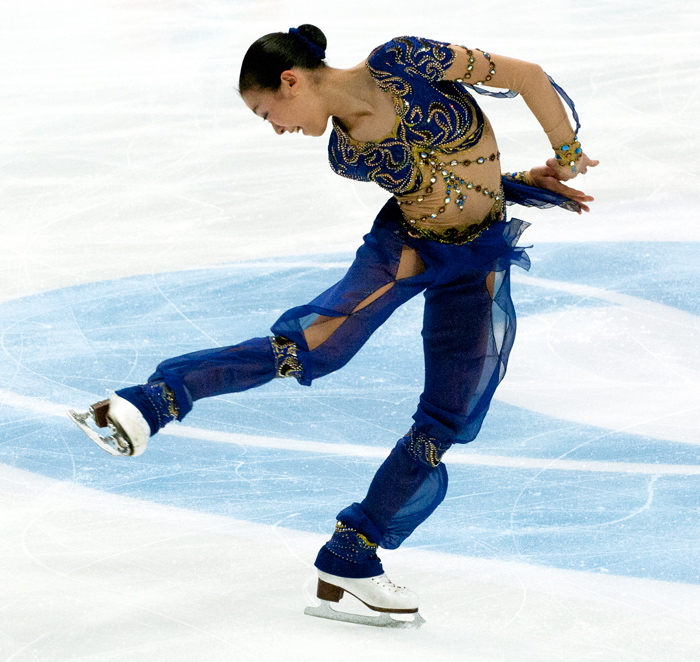
\includegraphics[width=10cm]{Spin/asada.jpg}
\caption{日本花样滑冰选手:浅田真央。}
%\label{default}
\end{center}
\end{figure}

\subsubsection{静止的陀螺}

首先先让我们由一个静止的陀螺开始:

陀螺一头大、一头小,小的一端非常尖,如果我们能够,仅仅是假设让物体的重力通过尖端的话,陀螺即便静止也能够立在支撑点P上。

但这个平衡是不稳定的,我们可以设想桌子的晃动,甚至人的呼吸都能扰动静止的陀螺,使其偏离平衡,然后重力就会使陀螺倒下。但严格说不是重力使陀螺倒下,因为支撑力是能够和重力抗衡的,使陀螺倒下的是力矩,支撑力向上,重力向下,而两个力现在又对不上,这就像两手转动方向盘,向相反的方向用力,总的效果就是方向盘转动起来了。当然这个运动无法持久,陀螺轰然倒地,就像推倒一个立起来的条石。

\begin{figure}[htbp]
\begin{center}
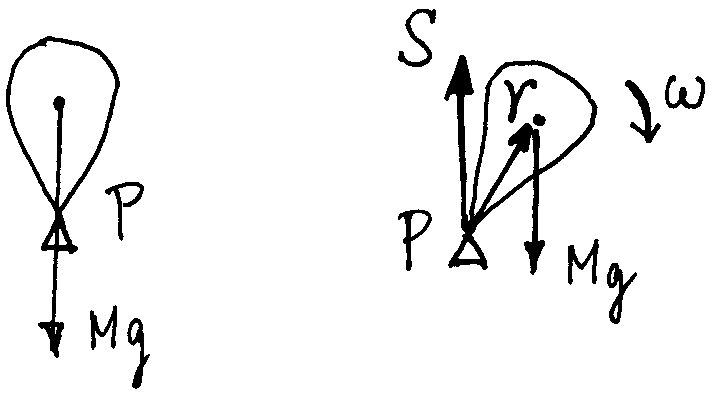
\includegraphics[width=8cm]{Spin/afallingspin.png}
\caption{静止的陀螺会倒下}
%\label{default}
\end{center}
\end{figure}

这种不稳定是很常见的现象,我们把它看作是正常的,是符合直觉的。比如一块立起来的条石,我们轻轻一推它就会倒。

但人呢?从形状上说人接近条石,照道理也是一推就倒,但推倒人要比推倒条石难,因为人是有“灵魂”的,他会根据推力调整自己身体的姿态,人是不太容易被推倒的,但原则上我们加大力,还是可以做到的。

\subsubsection{旋转起来的陀螺}

现在我们让陀螺围绕自身的轴转动起来。其实我们一般讲陀螺的运动,指的都是转动起来的陀螺,而且陀螺本身应该是具有轴对称性的,即陀螺围绕对称轴转动任何角度,在我们看来是一样的。

\begin{figure}[htbp]
\begin{center}
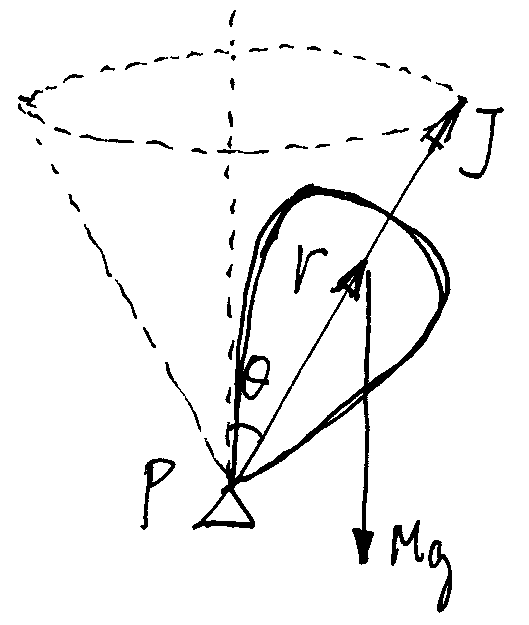
\includegraphics[width=5cm]{Spin/spinningtorque.png}
\caption{旋转起来的陀螺}
%\label{default}
\end{center}
\end{figure}

一个旋转起来的陀螺就是稳定的了,它可以稳定地立在它的尖端。假如我们稍稍偏转陀螺的转轴,陀螺并不会倒下去,它会倔强地以一个稍稍偏离垂直于地面的轴线继续旋转。

~

“陀螺的运动”对我们来说大有象征意义。

首先这是一个违反我们直觉的运动,在我们的直觉中一个歪着的物体,并且是大头朝上,小头朝下,仅凭一个点P与桌面接触,它就应该是不稳定的,它应该与万物一样有向下的趋势。但它偏不!

正因为陀螺行为的反常,所以它才显得好玩,甚至是由灵性的,或接近于神圣的。

在古希腊的观念里,诸天是最神圣的,它们最完美,最善,而最完美最善的几何形体就是“球”。这是爱利亚学派巴门尼德的观念,翻译成现代语言就是球具有最多的对称操作的数目(所谓对称就是某个操作下的不变性,球在任意围绕球心的转动操作下都是不变的),因此它是最完善的。

巴门尼德说的其实不是球,它说的是围绕固定轴旋转起来的球,即天文学意义下的“诸天”。我们现在就知道为什么陀螺是神圣的了,因为它是对神圣诸天的模仿,但它在现实中,在万物皆会腐朽变化的地界,因此它终将会停止旋转,屈服于必朽物向下的趋势,因为各种阻力,各种不够理想的原因。

陀螺是能模仿诸天运行的物件,而且就在我们的身边,可以随身携带,放在兜里面。于是我们看到在电影《盗梦空间》中,梦和现实的区分也是依靠一个旋转的陀螺。梦境是理想的世界,那里的陀螺永不倾倒。而在现实世界里,不论陀螺转的多快,终有倒下的一刻,即人的灵魂、人的意志终有抵挡不住朽坏和变化的那一刻。

\begin{figure}[htbp]
\begin{center}
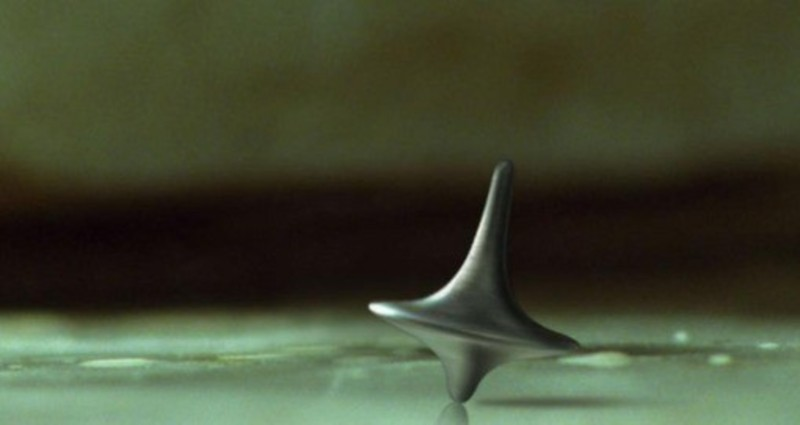
\includegraphics[width=8cm]{Spin/spinningtop.jpg}
\caption{盗梦空间里的陀螺}
%\label{default}
\end{center}
\end{figure}

\subsubsection{陀螺的进动}


旋转起来的陀螺,一般而言会参与两个运动,一个是陀螺自身围绕其对称轴的高速转动,这种转动可以被说成是自己围绕自己的旋转,它看起来是不动的,因此也就有柏拉图在《理想国》第四卷中的著名段落。

\begin{figure}[htbp]
\begin{center}
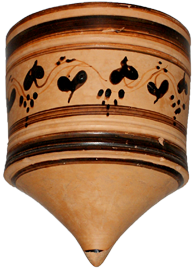
\includegraphics[width=8cm]{Spin/ivyleavestop.png}
\caption{出土于底比斯(Thebes)的公元前5世纪的陀螺,陀螺上装饰有常青藤叶图案。陀螺是当时妇女、儿童喜爱的玩具,同时也是向神献祭的贡品。在观念上旋转的陀螺是对神圣诸天的模仿。}
%\label{default}
\end{center}
\end{figure}


柏拉图说“我们不能讲陀螺既是动的,又是不动的”这种不合逻辑的话,(字面上看这和“波粒二像性”很像)。要说就要说明白,柏拉图采用的方案是“分类”,即把陀螺的运动——这一完整的运动——分解为轴线部分和非轴线部分,他说陀螺的轴线部分——假设陀螺的轴线垂直于地面——是静止的,而陀螺的非直线部分在运动,在三维空间中运动。

更严谨的讨论是:假设陀螺的运动是定点转动,对“陀螺的支撑点”,和“陀螺的非支撑点”分别讨论其运动,陀螺的支撑点是定点因此是不动的,而陀螺的非支撑点部分则是动的。

陀螺除参与围绕自身对称轴的转动外,陀螺整体还会围绕垂直于地面的轴线转动,这个运动和陀螺本身围绕其对称轴的运动不是一个运动,我们一般称之为进动。

即陀螺一边围绕自己转,一边其整体围绕着垂直于地面的轴线转动。陀螺与地面的非垂直的夹角$\theta$会给陀螺一个力矩,这个力矩正好驱动陀螺围绕垂直于地面的轴进动。

在我看来这些运动都是很难想象的,以上是对现象的描述,而要理解这个现象借助于力矩、角动量等自然很简单,但要能够想象这种运动并不容易,这就是我说的反直觉。

陀螺所受力矩是:

\begin{equation}
\tau = Mg r \sin \theta
\end{equation}

假设经过了$\Delta t$时间,陀螺围绕自身轴线高速旋转具有角动量$J$,角动量$J$会以某个角频率$\Omega$围绕垂直于地面的轴线进动。

$\Delta t$时间内,角动量的改变是:

\begin{equation}
\Delta J = J \sin \theta \Omega \Delta t
\end{equation}

最后“力矩乘以时间 = 角动量的改变”,即:

\begin{equation}
\tau \Delta t = \Delta J
\end{equation}

我们可以求出陀螺进动的频率:

\begin{equation}
\Omega = \frac{Mg r}{J}
\end{equation}

我们的结论是,如果陀螺转的越快的话,角动量$J$也就越大,相应地进动频率会比较小。

陀螺是一种反直觉的运动,所谓“反直觉”就是和我们的“想当然”的猜测正好相反。这些都与“旋转”有关,如果翻检物理学史的话,我们能找到不少这样的例子。

\begin{enumerate}
\item 

围绕不同转轴的转动没法交换次序。比如我们先围绕$x$轴旋转$90^o$,然后围绕$y$轴转动$90^o$这一系列的旋转操作和先围绕$y$轴转动$90^o$再围绕$x$轴旋转$90^o$是不一样的。(我们约定所有转动都是逆时针转动)

写成代数式子就是:

\begin{equation}
R_y (\pi /2)  R_x (\pi/2)  \neq  R_x (\pi/2)  R_y (\pi /2)
\end{equation}

这就导致了非对易代数。(其实就是把转动这种操作对应到一种数学语言/结构中去)

\item 

福科摆,假设地球不围绕自己旋转的话,我们是观察不到单摆轨迹的花样的。

\item

电子的托马斯进动。

\end{enumerate}

\subsubsection{惯性导航}

陀螺有一些变种,比如旋转的子弹,它一旦旋转起来,就不会因风等因素使子弹翻转,而保持大致固定的取向。(用物理的语言说就是,假如物体有个大角动量的话,你要改变它的取向$\theta$,你就需要给它一个足够大的力矩。)

\begin{figure}[htbp]
\begin{center}
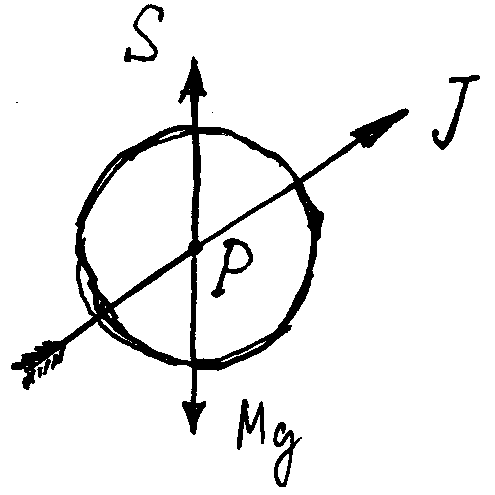
\includegraphics[width=5cm]{Spin/rotationofaball.png}
\caption{陀螺仪原理}
%\label{default}
\end{center}
\end{figure}

可以设想一个飞速旋转的均匀球体,我们假想在球的重心处施加一个向上的力,或我们在想象中把支点固定在球的球心处,所谓支点有两方面的作用,一是支撑,一是固定使其可以被我们带着走来走去。

现在所有的力都是通过支点施加给球的,除此之外它将不受任何外力,因此没有任何力矩会施加在这个球上,因此球的角动量将保持不变。大小和方向都不变,换句话说球的取向将永远不变,不管支点如何动的热闹。

这就是惯性导航的原理,如果我们让这个球高速转起来,并让它的转轴指向某个方向,这个方向将和我们如何运动支点P无关,它永远指向那个固定方向。在此意义下我们的陀螺确实是对神圣诸天的模仿,我们天球的转轴大致是指向北极星方向的。

当然地球并不是一个理想的陀螺,因为它本身的质量分布并不完全对称,这导致了力矩不能完全为0,这导致了地球转轴的方向其实有进动。

这个效应非常小。天文学上叫岁差,一个中等长度的周期是25868年,相比于人生百年,这个变化实在太小了,完全可以忽略。

人类其实很早就发现岁差了,古希腊的天文学家喜帕恰斯(约前190年-前120年)是一个毫不逊色于第谷的古代天文学家,他在比较了他的数据和古巴比伦人的数据后发现了岁差,这再次提示我们科学是一项超越个人生死的集体的事业,若无共同的信仰,持续的观测,岁差或地球自转的进动就不可能被观测到。知识的进步则更加无从谈起。

~

不使用数学,陀螺是一种很难被想象的运动,这一方面使陀螺成为人们好奇的对象,从而成为大人、小孩玩耍的玩具,同时陀螺也保有了一份神秘,就像我们面对星空时的感觉一样,一方面她(现象)是向我们敞开的,我们为之吸引,研究她接近她,但另一方面她又是向我们封闭的,永远向我们保留一部分秘密,提醒我们天与地、永恒与必朽、我与物的区别。(这符合古希腊哲学中对知识、对智慧的定义,我们可以接近她,有认识她的能力,但我们永远处在饥渴和追求的过程中,成为神或全知全能的可能性对人来说是封闭的。)

\begin{figure}[htbp]
\begin{center}
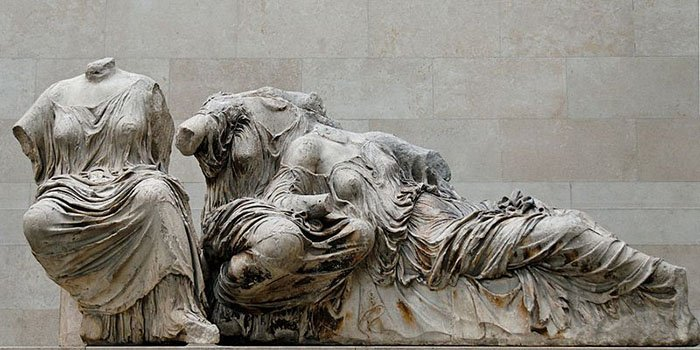
\includegraphics[width=10cm]{Spin/threegoddess.jpg}
\caption{命运三女神雕像:一个女神转动纺轮纺线,一个女神丈量线的长度,一个女神剪短绳子。纺轮的运动也是一种自己围绕自己的转动。}
%\label{default}
\end{center}
\end{figure}

我们现在不知道陀螺是受何种“机械”启发的,纺轮很可能启发了陀螺的发明。或者说纺轮的对象化,去功能化就是陀螺,即陀螺是废弃的纺轮,成为妇女和小孩纯粹娱乐/玩耍的对象。柏拉图在《理想国》第十卷中曾提到过一个关于宇宙的模型,就是基于纺轮、纺杆和挂钩的图像。

\begin{figure}[htbp]
\begin{center}
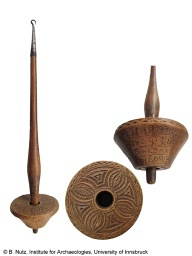
\includegraphics[width=5cm]{Spin/thespindle.jpg}
\caption{古希腊的纺轮、纺杆和挂钩。}
%\label{default}
\end{center}
\end{figure}

\subsection{电子的发现}

电现象是很古老的一种现象。毛皮摩擦橡胶棒带的是负电,玻璃摩擦丝绸带的是正电。我们可以通过接触的方法把电“接”到纸屑上做实验,发现同性相斥,异性相吸,我们还可以把电接到“量电器”上,量电器有两个脚,两个脚因解除都带同性的电,电越多,两个脚的夹角就越大。

关于电的最早的模型是“双流体模型”,所谓流体就是水流,水流可以流来流去,电也可以流来流去,正电和负电分别对应两种流体。但从哲学上假设两种实体是让人不舒服的,比如奥古斯丁就否定有恶的实体,他把恶解释为善的缺乏,或说只有善一种实体。受这种思想的影响,有人就提出单流体模型,把负电解释为正电的缺乏……

当然我们现在知道,有两种电荷,一种是正电,一种是负电……但这种把“负”解释为“正”的缺乏的idea后来在物理里还真用上了,比如狄拉克的“空穴”(hole)概念,所有“负能量”的电子的态都是填充满的,假如我们湮灭掉一个具有“负能量”的电子,就相当于产生了“正能量”的“空穴”,在充满“负能量”电子的背景上,并且电荷是亏空$-e$的,或换句话说我们可以把“空穴”看做是个带相反电荷$e$的正电子,电子的反粒子。

~

现在我们回到对电现象的讨论,牛顿的万有引力定律后,受此启发,大家猜想对电现象应该也有这么一个平方反比的定律,即力的大小正比于距离的平方分之一($F \propto r^{-2}$),两电荷离得越近力越强,越远力越弱。平方反比规律是很直观的,假如我们的空间是三维的,假如我们的质点、电荷会向空间的各个方向放出力线,或散发出某种神秘的“诱惑”,这个力线或诱惑是不应该无缘无故地消失的,它们同时向空间的所有方向跑,假如距离质点或电荷$r$地方我们做一个球面截住这些力线,在这个距离上我们能感受到相互作用的强弱应该正比于力线的密度,即单位面积里力线的“根数”,力线的根数和电荷或质量有关(或更直观地说一个电子或一个质量子放出一根“力线”),而单位面积就是要除以这个同心球面的面积($4 \pi r^2$),力线的密度就是场的强度,假如我们在这个地方再放上另外一个电荷,力的大小就是:

\begin{quote}
场的强度乘以电荷,
\end{quote}

完整写出来:$F \propto \frac{q_1 q_2}{r^2}$。这个力就是库伦力,因为库伦最早做了这个实验,并把比例系数定下来……写成国际单位制就是:

\begin{equation}
F = \frac{1}{4 \pi \epsilon_0 } \frac{q_1 q_2}{r^2}
\end{equation}

这里$\epsilon_0 = 8.854 \times 10^{-12} F/m$,是真空介电常数(Vacuum permittivity)。

~

在原子论的观念下,人们自然会猜测对电现象而言有电的原子。即存在着很小很小的带电的基本单元,甚至我们会把这个基本单元想象为一个小圆球,很多小圆球在一起,看起来就像是一种流体,或用现代的概念讲就是一种“颗粒流”。

在牛顿力学之后,人们有一种对世界的想象,或一种关于世界的整体图景,在这个图景下,世界就是一个质点系统,很多很多质点,质点间有相互作用,在某一刹那($t = t_0 $ ),每个质点的位置和速度(或动量)都是确定的,这时我们就面对一个巨大的联立方程,对每一个质点都是个牛顿第二定律,比如对第$i$个质点:

\begin{equation}
F_i = \sum\limits_{ j \neq i } F_{ij}    =  m a_i
\end{equation}

$F_{ij}$表示第$j$个质点给第$i$个质点的力。但这里力是什么?即质点和质点的相互作用是什么?如果从前的话就是万有引力定律,但现在又多了库伦力,库伦力不同于万有引力的是,第一它可能是吸引的也可能是排斥的,而引力就只能是吸引的,单纯靠引力,世界是不稳定的。第二电磁相互作用,或这里就是库仑力,比引力要强的多,光靠引力我们甚至解释不了最简单的物质——比如氢原子——的结构,但有电磁相互作用就可以。

我们知道有四种相互作用,或三种,引力最弱,强相互作用最强,但它仅存在于原子核里面,剩下的就是“电磁相互作用+弱相互作用”(统称“电弱”,用一套理论描述),我们所处的这个层次的世界,比如为什么会有生命等等,主要是用电磁相互作用解释的。

传统上讲,化学是研究物质结构的。在电化学实验中,我们可以电解水,电解盐酸……

\begin{eqnarray*}
2 H_2 O & \to & 2 H_2 \uparrow + O_2 \uparrow  \\
2 H Cl & \to &  H_2 \uparrow + Cl_2 \uparrow
\end{eqnarray*}

在这些实验中我们会发现产生单位质量的氢气(比如2克)总和确定量的氧气(8克)和确定量的电量转移(1F)相匹配。这提示我们电很可能存在一个最小单元,这个最小单元参与化学反应,它使比如两个氢离子变成一个氢气分子($2 H^+ + 2 e \to H_2  \uparrow $)。并且这个基本单元普遍存在于很多物质中。

~

在发现电子的过程中,塞曼效应(Zeeman effect)是很关键的。所谓塞曼效应就是研究磁场对光的影响,这是法拉第(Faraday,1791 — 1867)临终时研究的课题,但由于他当时用的磁铁不够强大,他没看到磁场对光的任何影响。

法拉第一生做了很多实验,记了好多实验笔记,他的工作奠定了电磁场理论的实验基础。麦克斯韦是电磁理论的数学形式的完成者,所谓场就是物理量(这里就是电场强度$E$/磁场强度$B$)在空间中的分布和时间上的变化,电场和磁场必须看做是个整体,而电场/磁场本身又是矢量,在三维空间上有分量,可以想象电磁场的理论是很复杂的。

麦克斯韦的理论证明光其实就是一种电磁波,一种肉眼可以看见的电磁波,光波波长正好对应太阳——我们的母星——发出的主要电磁辐射。这不是巧合,我们的母星以黄光照亮我们的世界,我们人类的视觉器官也主要适应这个波长,并在这个波长附近进化出辨认不同波长的能力——通过颜色——赤橙黄绿青蓝紫。颜色使我们一眼就能从环境获得更丰富的信息,进而通过生活造就我们内在的心理和智力世界,眼睛充分利用了太阳给我们的馈赠,发达的视觉是人类演化出智慧的基础。

~

牛顿用三棱镜可以把不同波长的光分开,这就是最原始的光谱(spectrum),所谓谱就是分布,光谱就是光强随不同波长的分布($I_{\lambda}$),但牛顿的方法分辨本领不高。

更好的——把不同波长的光分开的方法——是利用光的干涉现象,假如有两束光它们都是从A出发走不同路径,最后都落在屏上的B,如果它们走过的路正好相差波长$\lambda$的整数倍的话,它们就会波峰和波峰叠加,对应光的加强,即一个明亮的条纹,换句话说条纹的位置会和波长的长度有关,不同波长的光会在屏的不同位置出现加强(他强你不强,你不强他强)。现在的问题是要让条纹们变窄一点,否则都叠在一起不好测量。

我们可以使用光栅来使条纹变窄,所谓光栅就是把光分成细而密集的很多束,比如最早的光栅就是用金属丝缠绕而成的,而晶体因为本身就有周期性结构,可以看做是天然的光栅。

假设有很多束光,它们两两之间正好相差$\delta$相位$e^{i \delta}$,所有这些波的叠加是:

\begin{equation}
1 + e^{i \delta} + e^{i 2 \delta } + ... + e^{i N \delta}
\end{equation}

这是一个等比数列,我们可以求出和是:

\begin{equation}
\frac{1 - e^{i N \delta}}{ 1 - e^{i \delta}} = \frac{ 1- \cos N \delta - i \sin N \delta }{ 1- \cos \delta - i \sin \delta}
\end{equation}

光强正比于波幅的绝对值的平方:

\begin{equation}
I(\delta) \propto \frac{( 1 - \cos N \delta)^2 + \sin^2 N \delta  }{  (1 - \cos \delta)^2 + \sin^2 \delta } = ... = \frac{\sin^2 N\delta /2}{\sin^2 \delta /2} 
\end{equation}

可见增加$N$会有效地提高光栅的分辨本领,随着光栅技术的进步,我们能够把不同波长的光在光谱上分的越来越开。

~

与此同时洛伦兹基于麦克斯韦的电磁场理论提出了他的关于金属的理论,他假设金属里面有很多带电的基本粒子,它们和分子运动论中讨论的原子一样在做无规则的热运动,在这样一幅图像下洛伦兹解释了电的输运现象,比如为什么会有欧姆定律(Ohm's law)。

塞曼是洛伦兹的助手,他受法拉第想法的启发,想再试一试磁场对光的影响,当时实验技术已经有很大进步了,更大的磁铁,更精细的对光波波长的分辨等等。塞曼对磁场中的钠光谱进行了分析,发现磁场能够使钠的黄线变粗(就是分裂了),他测量了波长的变化,并把结果告知洛伦兹。

洛伦兹很快基于他的电子论给出了对塞曼效应的解释。假设金属里面有带电的基本单元,这个基本单元的运动对物性负责,现在磁场加上去了,就有洛伦兹力$q v B$,洛伦兹力是有方向的,假设带电粒子既可以围绕磁场顺时针转动,也可以逆时针转动,这个力对顺时针转动和逆时针转动的影响就是相反的,它使得一个转动变快,而使另一个转动变慢。转动快慢对应频率,而频率对应波长。

\begin{equation}
\lambda = c T = \frac{c }{\nu} = \frac{2 \pi c}{ \omega }
\end{equation}

洛伦兹基于以上思路做了一个简单的计算,正好可以解释塞曼的实验结果。并且给出了一个重要的结果,假如金属中的这个带电单元既有质量($m$)又有电荷($q$)的话,它们的比值将是$q/m \propto 10^{11} $库伦/千克。

几个月后,JJ汤姆逊就对阴极射线完成了他的著名实验,在这个实验中他对阴极射线的轨迹进行了直接的测量,阴极射线在磁场的作用(洛伦兹力)下会偏转,这用粒子图像很容易解释。汤姆逊测出了阴极射线的电荷质量比,也是大约$10^{11}$库伦千克。

关于存在电的基本单元,我们现在就有了好几个独立的证据,电解实验表明在水、盐酸……中存在着带电的基本单元,塞曼效应说明在金属中存在带电的基本单元,汤姆逊实验说明在阴极射线里有带电的基本单元,而且我们还观察到了带电基本单元在磁场和电场下的偏转,这可以说是更直接的证据。

现在汤姆逊就假设在物质中普遍存在带电的基本单元,并称之为电子,它是负的,电荷质量比是$10^{11}$库伦/千克量级。汤姆逊还猜测,如果存在带正电的基本单元的话,其电量应该和带负电的基本单元——电子——相同,只是正负号相反。这个猜测是合理的,因为在电解水实验里就是电子在离子之间跑来跑去,这意味着一个氢离子(质子)加一个电子正好就是电中性的。

\begin{eqnarray*}
2 O^{--} & \to &  O_2 \uparrow + 4 e \\
4 H^+ + 4 e  & \to & 2 H_2 \uparrow 
\end{eqnarray*}

我们也可以用磁场偏转质子来测量质子的电荷质量比$e/m_p$,发现这个数比电子的电荷质量比小很多,说明电子比质子轻很多。这个结果让我们很不舒服,因为自然界中带负电的基本单位竟然比带正电的基本单位轻很多……假如质量一样,只是电荷相反我们就会觉得舒服,有“左右对称”式的“均衡”感。现在我们知道有电子有反电子,有质子也有反质子,这就舒服多了,于是问题就变成为什么我们的这个世界电子会比反电子多很多……,这个问题是被苏联物理学家萨哈罗夫解决的。

密立根通过油滴实验测出电子电荷的具体数值$e = 1.602 \times 10^{-19} C$,这意味着现在电子的质量也知道了$m_e = 9.109 \times 10^{-31} kg$。

那么电子有多大呢?我们现在有两个简单的选择,一种是把电子想象为一个球体,它的半径是$r_e$,电荷和质量都均匀地分布在这个球体上。另一种选择是把电子干脆看成是一个点,好比曾经的质点模型,我们用位置和速度描述电子的运动状态(或在量子力学中,以位置和时间为变量的波函数$\psi(x,t)$),就电子本身而言,它的质量是$m_e$,电荷是$e$(虽然说电子带负电,但我们还是习惯把它写为$e$,这里的逻辑很简单,就是省事)。

~

回到塞曼效应,进一步的实验表明,塞曼效应比我们想象的复杂,我们可以把不同的金属放进磁场里,测不同的谱线分裂。我们发现谱线可能会分裂成偶数条,这是洛伦兹粗糙的电子论无法解释的。我们把理论上好解释的叫“正常塞曼效应”,把暂时还没法解释的起名叫“反常塞曼效应”。但实际上大部分观察到的是“反常塞曼效应”,或者说你们“正常”的其实才是“反常”的。

塞曼效应(磁场中光谱线的分裂)是原子物理中的一个重要实验,因为它很早就发现了,一直没获得完满的解释,或者说它一直在驱动理论演进。此外塞曼效应还启发人们去研究电场中光谱线的分裂,这就是斯塔克效应(Stark effect),斯塔克效应对催生量子力学也有重要作用。

~

根据物质的摩尔质量,密度等参数我们可以估计不同元素原子的大小,其结果非常整齐,都是$10^{-10}$米,即不管它们的密度多么悬殊,但对于构成它们基本单元的原子,不同种类原子的大小是差不多的。

\begin{table}[htdp]
\begin{center}
\caption{不同原子的半径}
\begin{tabular}{|c|c|c|c|}
\hline 
元素&   质量数$A$&    质量密度$\rho$($g / cm^3$)&
原子半径($nm$)\\
\hline
Li &  7&  0.7&   0.16\\
Al & 27& 2.7& 0.16\\
S &  32& 2.07&    0.18\\
Cu &  63& 8.9&    0.14\\
Pb &  207& 11.34&    0.19\\
\hline
\end{tabular}
\end{center}
\end{table}

我们还可以估计电子的大小$r_e$,根据狭义相对论,质量就是能量,能量就是质量,电子的质量$m_e$对应能量$m_e c^2$,而电子本身还带电荷$e$,电荷周围是电场的分布,假设电荷是个半径为$r_e$的均匀带电球体的话,我们能把电场在整个空间的分布$E(r) $都计算出来,根据电磁学,电场是有能量的,单位体积的能量(或能量密度)是$ \frac{\epsilon_0}{2} E(x)^2$,我们把所有电场的能量都加起来,它将是一个和参数$r_e$有关的表达式,这样表达出的能量要和电子的总能量$m_e c^2$相等。相当于我们从两个角度计量了电子的总能量,然后我们就能计算出$r_e$。

这样计算出来的$r_e$很小,大约是$10^{-15}$米,它比原子的尺度$10^{-10}$米小很多,就相当于我们在足球场里爬进了一只小蚂蚁。

这个计算很微妙,首先它似乎否定了电子——是个几何点——这样的物理图像(因为这样的话总能量会趋于无穷大),其次它是通过考虑相对论来否定的。这意味着我们必须考虑相对论才能得到一个关于电子的完整理论。这也是当时物理学家的普遍想法,因为狭义相对论1905年就提出了,把所有物理理论推广使其符合相对论是当时很多理论家喜欢做的事情。

我们还知道电子不是经典的对象,我们必须发展量子力学的理论才能描述它的运动,假如电子的运动速度很慢,也许存在一个非相对论性的量子力学,但如果电子的运动速度接近光速,就必须使用相对论性的量子力学。

当时很多物理学家都希望能直接得到一个关于电子的相对论性理论,但最后都失败了。首先成功的还是一个关于电子的非相对论性理论,即海森堡-玻恩-约丹的矩阵力学和薛定谔的波动力学。

\begin{figure}[htbp]
\begin{center}
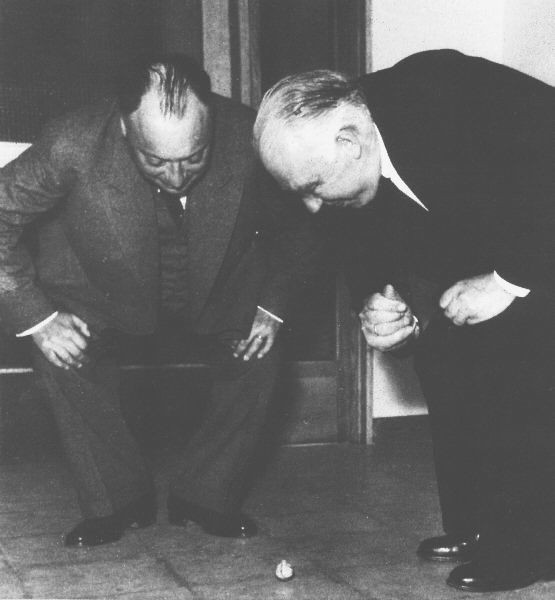
\includegraphics[width=6cm]{Spin/bohrandpauli.jpg}
\caption{玻尔和泡利在一起玩陀螺。}
%\label{default}
\end{center}
\end{figure}

在非相对论性量子力学中,电子是被当做点处理的,因为把电子处理为球体,并认为电子会像地球一样自转起来恰恰无法解释反常塞曼效应。我们必须接受这样一个尴尬的局面——我们把电子理解为点,但同时这个点还必须能有角动量(自旋角动量$s$)和磁矩。这是非常别扭的,我们在经典物理中根本就找不到这样的例子\footnote{这是柏拉图在《理想国》第四卷中讨论的问题,对于一个点我们能说它围绕自身旋转吗?

柏拉图否定了点能旋转,用我们今天的话说就是“对于一个几何的点,没有自转,只能是静止的”。

那什么是转动呢?

如果我们把转动定义为物体的一部分相对于另一部分在空间中的运动的话,我们就可以立刻说对于点是不可能有自转的,因为它没有部分(点在《几何原本》中的定义是“没有部分”)。

更多请参考:“柏拉图、陀螺和自旋”, \url{http://jianshu.io/p/3f98e4086955} }。

如果我们回顾海森堡等创建量子力学的过程的话,他们非常依赖于把原子现象(量子力学)与日常经验(经典力学)进行类比,他们建立了一整套对应的法则,根据这些法则,我们由经典力学的概念、公式出发就会得到相应量子力学的概念、公式。比如经典力学中的位置$r$对应量子力学中的位置算符$\hat r$;经典力学中的角动量$L$对应量子力学中的角动量算符$\hat L$;经典力学中的泊松括号对应量子力学中的对易关系等等。

这里我们碰到的就是这个困难——自旋角动量$S$没有经典对应,它是个纯粹的量子现象,我们没法用一个陀螺的旋转(或任何其他经典现象)与之对应。

这个困难必须到狄拉克的相对论性量子力学才能得到解释,在那里电子仍然被当做一个点来处理,但这个点所满足的运动方程是个矩阵方程,它可以求出四个解,两个解是正能量,两个解是负能量。负能量解对应的是反电子(为了好理解,狄拉克把它解释为电子背景上的空位,即空穴,但到量子场论里我们是不需要借助这个图像的),而两个解分别对应自旋向上和自旋向下。电子和反电子在形式上现在就对称了,它们质量相同,什么都一样,就是电荷不同。

现在我们再来说电子的话,电子就是这样一个对象,它的自旋角动量是1/2,质量是$m_e$,电荷是$e$,电子本身的运动状态要用波函数来表示,但有两个分量,一个对应自旋向上,另一个对应自旋向下。我们可以把它写为列向量的形式:

\begin{equation}
\left(  
\begin{array}{lcr} 
\psi_{s \uparrow} \\
\psi_{s \downarrow}
\end{array}
\right)
\end{equation}


\subsection{自旋的发现}


有两种讲授量子力学的方法,一种是按照历史的逻辑,介绍黑体辐射、关电效应、康普顿散射、卢瑟福散射、玻尔模型、塞曼效应等一系列著名实验,说明经典物理是如何失效的,然后建立“波粒二像性”概念,即“像波一样的粒子”,然后我们用波函数、薛定谔方程来描述电子。

以氢原子为例,不考虑相对论,我们需要求解这样一个偏微分方程:

\begin{equation}
i \hbar \frac{\partial }{\partial t} \psi (r, t) = \left[ -\frac{\hbar^2 }{2m} \nabla^2 + V(r) \right] \psi (r, t) 
\end{equation}

还有一种讲授量子力学的方法是直接从某一个实验出发引入量子力学。比如费曼就是从假想的双缝实验出发建立量子力学的,讨论双缝实验的好处是方便和费曼发明的路径积分方法对接。除双缝实验外还有一个选择,就是通过讨论斯特恩-盖拉赫实验引入量子力学。

但首先,让我们讨论“磁矩在磁场中运动”。

\subsubsection{磁矩在磁场中运动}

所谓磁矩就是一个小磁针。假设一个小磁针放到磁场里,磁矩在磁场中不受力,但会受到力矩的作用,它会倾向于倒向和磁场平行的取向。

\begin{figure}[htbp]
\begin{center}
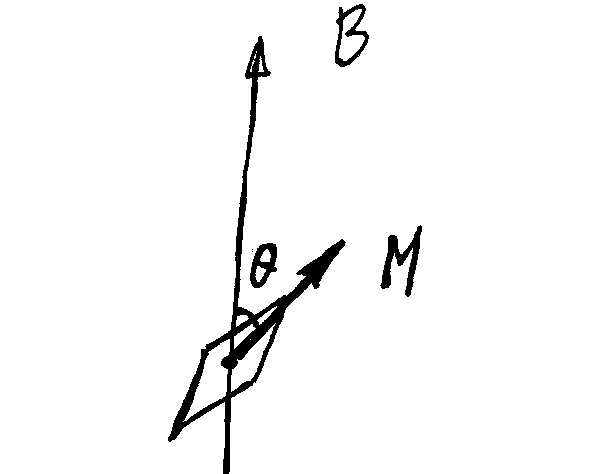
\includegraphics[width=4cm]{Spin/momentinB.png}
\caption{在磁场中的磁矩。}
%\label{default}
\end{center}
\end{figure}

假设磁针的磁矩是$M$,磁场是$B$,其能量为:

\begin{equation}
U = - B \cdot M
\end{equation}

类似于陀螺会在重力场中进动,磁矩也会围绕磁场进动。

力矩是:

\begin{equation}
\tau = \mu \times B = \frac{d J}{d t}
\end{equation}

这里$J$是角动量。

假设这里的磁矩$\mu $、角动量$J $都是“环形电流”导致的,即假设电子围绕$z$轴做圆周运动导致的磁矩和角动量。

\begin{figure}[htbp]
\begin{center}
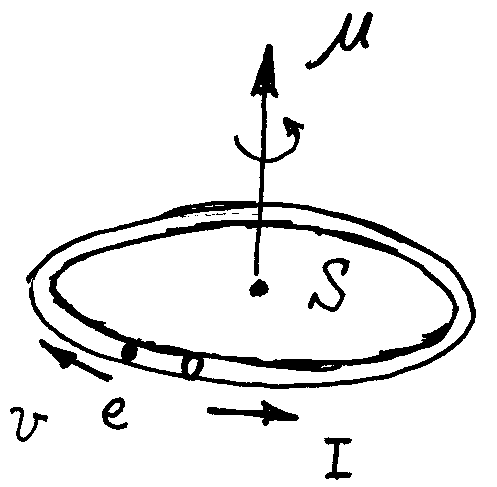
\includegraphics[width=5cm]{Spin/currentrotate.png}
\caption{电子的运动导致环形电流。}
%\label{default}
\end{center}
\end{figure}

角动量:

\begin{equation*}
L = r \times p =  m r^2 \omega 
\end{equation*}

磁矩$\mu$等于电流$I$乘以电流围成的面积$S$,电流是单位时间通过某截面的电荷数,即$I = \frac{\Delta Q}{\Delta t}$,如果取电子运行周期$T$是$\Delta t $的话,$\Delta Q$正好是电子的电量$- e$(负号表示电子带的电量是负的)。

现在:

\begin{eqnarray*}
\mu & = & IS = - \frac{e }{T } \pi r^2 \\
{} &=& - \frac{e}{2m} L
\end{eqnarray*}

换句话说电子的轨道运动会导致电子具有轨道运动的角动量(就像地球围绕太阳运动,地球会具有轨道角动量一样),同时电子是带电的,因此电子的轨道运动也会导致电子具有磁矩,就像一个环形电流会具有磁矩一样,因为都是电子的运动导致的,我们会发现磁矩和角动量是成正比的,我们把这个比例因子进一步改写为:$- g \frac{e}{2m}$,这里负号表示电子是带负电的,$g$是朗德因子,因为我们很快将发现电子不但具有轨道磁矩,它还将具有自旋磁矩。

字面上理解好像是说电子会同时参与两个运动,就像我们的地球在太阳系里的行为一样,一个是电子因轨道运动(这里就是半径为$r$的匀速圆周运动)导致的磁矩,另一个是电子因自旋运动(字面意思就是电子自己围绕自己旋转)导致的磁矩。对轨道运动而言$g_L = 1$,对自旋运动而言$g_S = 2$。写成统一的形式:

\begin{equation}
\mu = - g \frac{e}{2m} J
\end{equation}

我们用$J$表示一般的角动量,用$L$表示轨道角动量,$S$表示自旋角动量,当然马上我们会发现“自旋”(Spin)是个错误的命名。

在原子物理中我们用玻尔磁子(Bohr magneton, $\mu_B$)作为磁矩的单位:

\begin{equation}
\mu_B = \frac{e \hbar }{ 2 m} 
\end{equation}


%但为什么是2呢?

\subsubsection{斯特恩-盖拉赫实验}

我们可以通过讨论斯特恩-盖拉赫实验直接引入量子力学。

斯特恩-盖拉赫实验是个充满了意外的实验,斯特恩(Otto Stern)是爱因斯坦的第一个学生,但他却是个实验物理学家,他想用实验验证当时原子物理研究中的主流理论——“玻尔-索末菲模型”(Bohr-Sommerfeld model)。

玻尔模型是个大杂烩,为了解释原子光谱他把很多并不相容的假设捏在了一起。比如他让电子在一个轨道上围绕原子核运动,这就是经典力学。但他又引入了量子化条件,只允许电子在几个分立的轨道上围绕原子核运动,这就又不要经典力学了。

但既然玻尔模型能够很简单地解释氢原子光谱,而且推导又那么简单,物理学家认为这个对原子现象的描述还是很有潜力的,比如索末菲就对玻尔模型进行了推广。原子中电子和原子核之间符合库伦力,一个平方反比的吸引力,原子核本身的质量比电子质量大很多很多,这些都使得原子就像是一个微小的太阳系,根据开普勒的运动定律行星在一个椭圆轨道上围绕太阳运动,而椭圆是可以有不同偏心率的(圆是一种特殊的椭圆,偏心率为0)。

索末菲把玻尔模型中的圆轨道推广到椭圆轨道,同时他把玻尔的量子化条件也推广了。他引入了两个量子数,一个角量子数$n_\phi$,使:

\begin{equation}
\oint p_\phi d \phi = n_\phi h , n_\phi = 1, 2, ...
\end{equation}

这里$\phi$是电子在椭圆上运动时的方位角,$p_\phi = \frac{\partial L }{\partial \dot \phi }$,$L ( r, \phi; \dot r , \dot \phi  ) = T - V$是拉氏量。

另一个是径向的量子数$n_r$,使:

\begin{equation}
\oint p_r dr = n_r h , n_r = 0, 1, 2, ...
\end{equation}

使用极坐标系($r , \phi$)描述电子在原子核附近的位置,$r$是矢径,从原子核指向电子,$p_r$定义为$\frac{\partial L }{\partial \dot r }$。对正圆运动来说,$r$是个常数,所以$n_r$是可以等于0的。

\begin{figure}[htbp]
\begin{center}
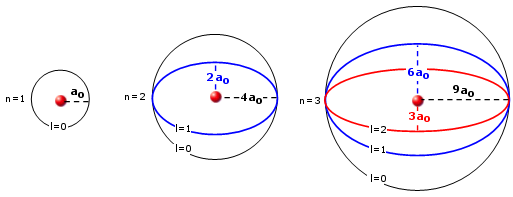
\includegraphics[width=11cm]{Spin/bohr-sommerfeld-model.png}
\caption{玻尔-索末菲模型,这里$l$相当于是$n_r$}
%\label{default}
\end{center}
\end{figure}




$n_r + n_\phi = n $,$n = 1, 2, 3, ...$就是原先玻尔模型中的量子数$n$(主量子数)。

\begin{table}[htdp]
\caption{玻尔-索末菲模型}
\begin{center}
\begin{tabular}{|c|c|c|c|}
\hline
主量子数$n$ & 角量子数$n_{\phi}$ & 磁量子数$m$ & 矢径量子数$n_r$ \\
\hline
1 & 1 & $\pm 1$ & 0 \\
\hline
2 & 2 & $\pm 2$ & 0 \\
{} & 1 & $\pm 1$ & 1 \\
\hline
3 & 3 & $\pm 3$ & 0 \\
{} & 2 & $\pm 2$ & 1 \\
{} & 1 & $\pm 1$ & 2 \\
\hline
\end{tabular}
\end{center}
\label{default}
\end{table}%


对$n = 1$而言,$n_\phi = 1$,$n_r$只能等于0。这是氢原子能量最低的态,称之为基态。考虑到电子既可以是顺时针围绕原子核运动,也可以是逆时针围绕原子核运动的,于是一个$n_\phi$就对应两个“状态”,用角动量的语言说就是$L = \hbar$,但角动量在$z$方向上的投影只能取$L_z = \pm \hbar $两种情况,即角动量的取向也是量子化的,只能沿$z$轴向上或向下。我们把$L_z$写作$m \hbar$,这里$m = \pm 1$,我们管$m$叫做磁量子数,只要$m$不是0,原子就会在$z$方向上有非0的磁矩。


量子化条件会引入不同于经典物理的陈述,比如能量分裂成一个一个能级——能量量子化;现在又导致角动量的$z$分量只能取分立值(对氢原子基态而言是两个),我们称这种现象为空间取向的量子化(Space quantization)。

%对$n=2$而言,$n_\phi = 1, 2$,$n_r = 0, 1$……

虽然“玻尔-索末菲模型”能解释不少物理实验,但对这么一个大杂烩式的理论,物理学家并不真的相信。比如电子是否真的会在原子里面按照圆形或椭圆形的轨道运动?这样的图像辅之以量子化条件等也许能够解释实验,但如果电子真的这么行为的话,那也太神奇了。

\begin{figure}[htbp]
\begin{center}
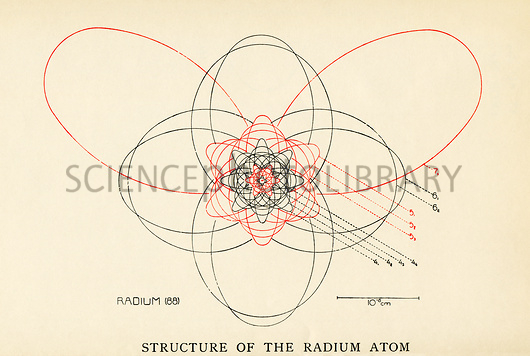
\includegraphics[width=10cm]{Spin/Bohr-Sommerfeld_model_of_the_atom.jpg}
\caption{玻尔-索末菲模型下的“镭”原子}
\label{default}
\end{center}
\end{figure}

斯特恩是物理化学的博士,但他却有幸成了爱因斯坦的第一个学生,作为犹太人,他的父母坚决资助他们的儿子继续深造。一战结束后,斯特恩又成了玻恩的助手,当时玻恩在法兰克福大学任教并领导一个实验室,在那里斯特恩研究了原子束方法。所谓原子束方法就是用一个炉子给金属加热,使金属原子从炉子里跑出来,通过准直装置后,然后再对射出来的金属原子进行各种操作和测量。

斯特恩知道要想验证氢原子的“空间取向量子化”,就要让$L_z = \pm \hbar$的基态氢原子分开,但如何把不同$L_z$的氢原子分开呢?斯特恩有一天醒早了,当时是冬天,他怕冷于是就躺在被窝里想这个问题。他想到可以让氢原子通过一个在$z$方向上的非均匀磁场$B(z)$,磁场的非均匀性可以通过磁场的梯度$\frac{d B(z)}{d z}$来描述,如果梯度足够大的话,就有可能把不同角动量的原子分开。

%%%%

假设原子的磁矩是$\mu$,它在磁场中的能量是:

\begin{equation}
U_m = - \mu \cdot B = \mu_x B_x + \mu_y B_y + \mu_z B_z 
\end{equation}

由于磁场是非均匀的,磁矩将会受到一个非0的力:

\begin{equation}
F = - \left( \hat x \frac{\partial }{\partial x} + \hat y \frac{\partial }{\partial y}  + \hat z \frac{\partial }{\partial z}  \right) U_m  = \hat z  \mu_z  \frac{\partial B_z }{\partial z}
\end{equation}

这里$\hat x $,$\hat y $,$\hat z $分别是$x, y$和$z$方向上的单位矢量,换句话说,原子受到的力在磁场的非均匀方向上,即$z$方向上,力的大小是:

\begin{equation}
F =  \mu_z  \frac{\partial B_z }{\partial z}
\end{equation}

可见这个实验的难点确实在磁铁上,磁铁的规格要使得$\frac{\partial B_z}{\partial z}$越大越好,同时磁铁要足够长,这样不同大小的力会驱动银原子在$z$方向上漂移足够长时间,使具有不同磁矩的原子充分分开。

%%%%

斯特恩有了这个想法后很兴奋,于是跑去向玻恩汇报,但玻恩并不认为这个实验有价值,在他看来“空间取向量子化”无非是个象征,在它的背后还有我们暂时不懂的物理,而斯特恩竟然在字面上相信会有这么回事,……,这就是他自己的事了\footnote{“It took me quite a time before I took this idea seriously. I thought always that (space) quantization was a kind of symbolic expression for something which you don’t understand. But to take this literally like Stern did, this was his own idea… I tried too persuade Stern that there was no sense (in it), but then he told me that it was worth a try.” 摘自:“Stern and Gerlach: How a Bad Cigar Helped Reorient Atomic Physics”,Physics Today 56, December 2003, \url{http://zimp.zju.edu.cn/~xinwan/qm2/note/PhysToday_Friedrich03.pdf}}。

斯特恩获得了盖拉赫的帮助,而盖拉赫直到此时才第一次听说“空间取向量子化”。实验很难做,花了斯特恩和盖拉赫一年多时间。

他们使用的是银原子Ag,用炉子把银加热到1000多摄氏度,然后使跑出来的银原子通过两个只有0.03毫米宽的准直装置。磁铁有3.5厘米长,磁场强度是大约0.1特斯拉,在$z$方向上的梯度达到了10特斯拉每厘米。银原子确实分裂成了两束,两束的间隔只有0.2毫米,而准直装置或磁铁的方位只要差0.01毫米就会把银原子的分裂图样破坏掉。可想而知这是一个十分精细的实验。

\begin{figure}[htbp]
\begin{center}
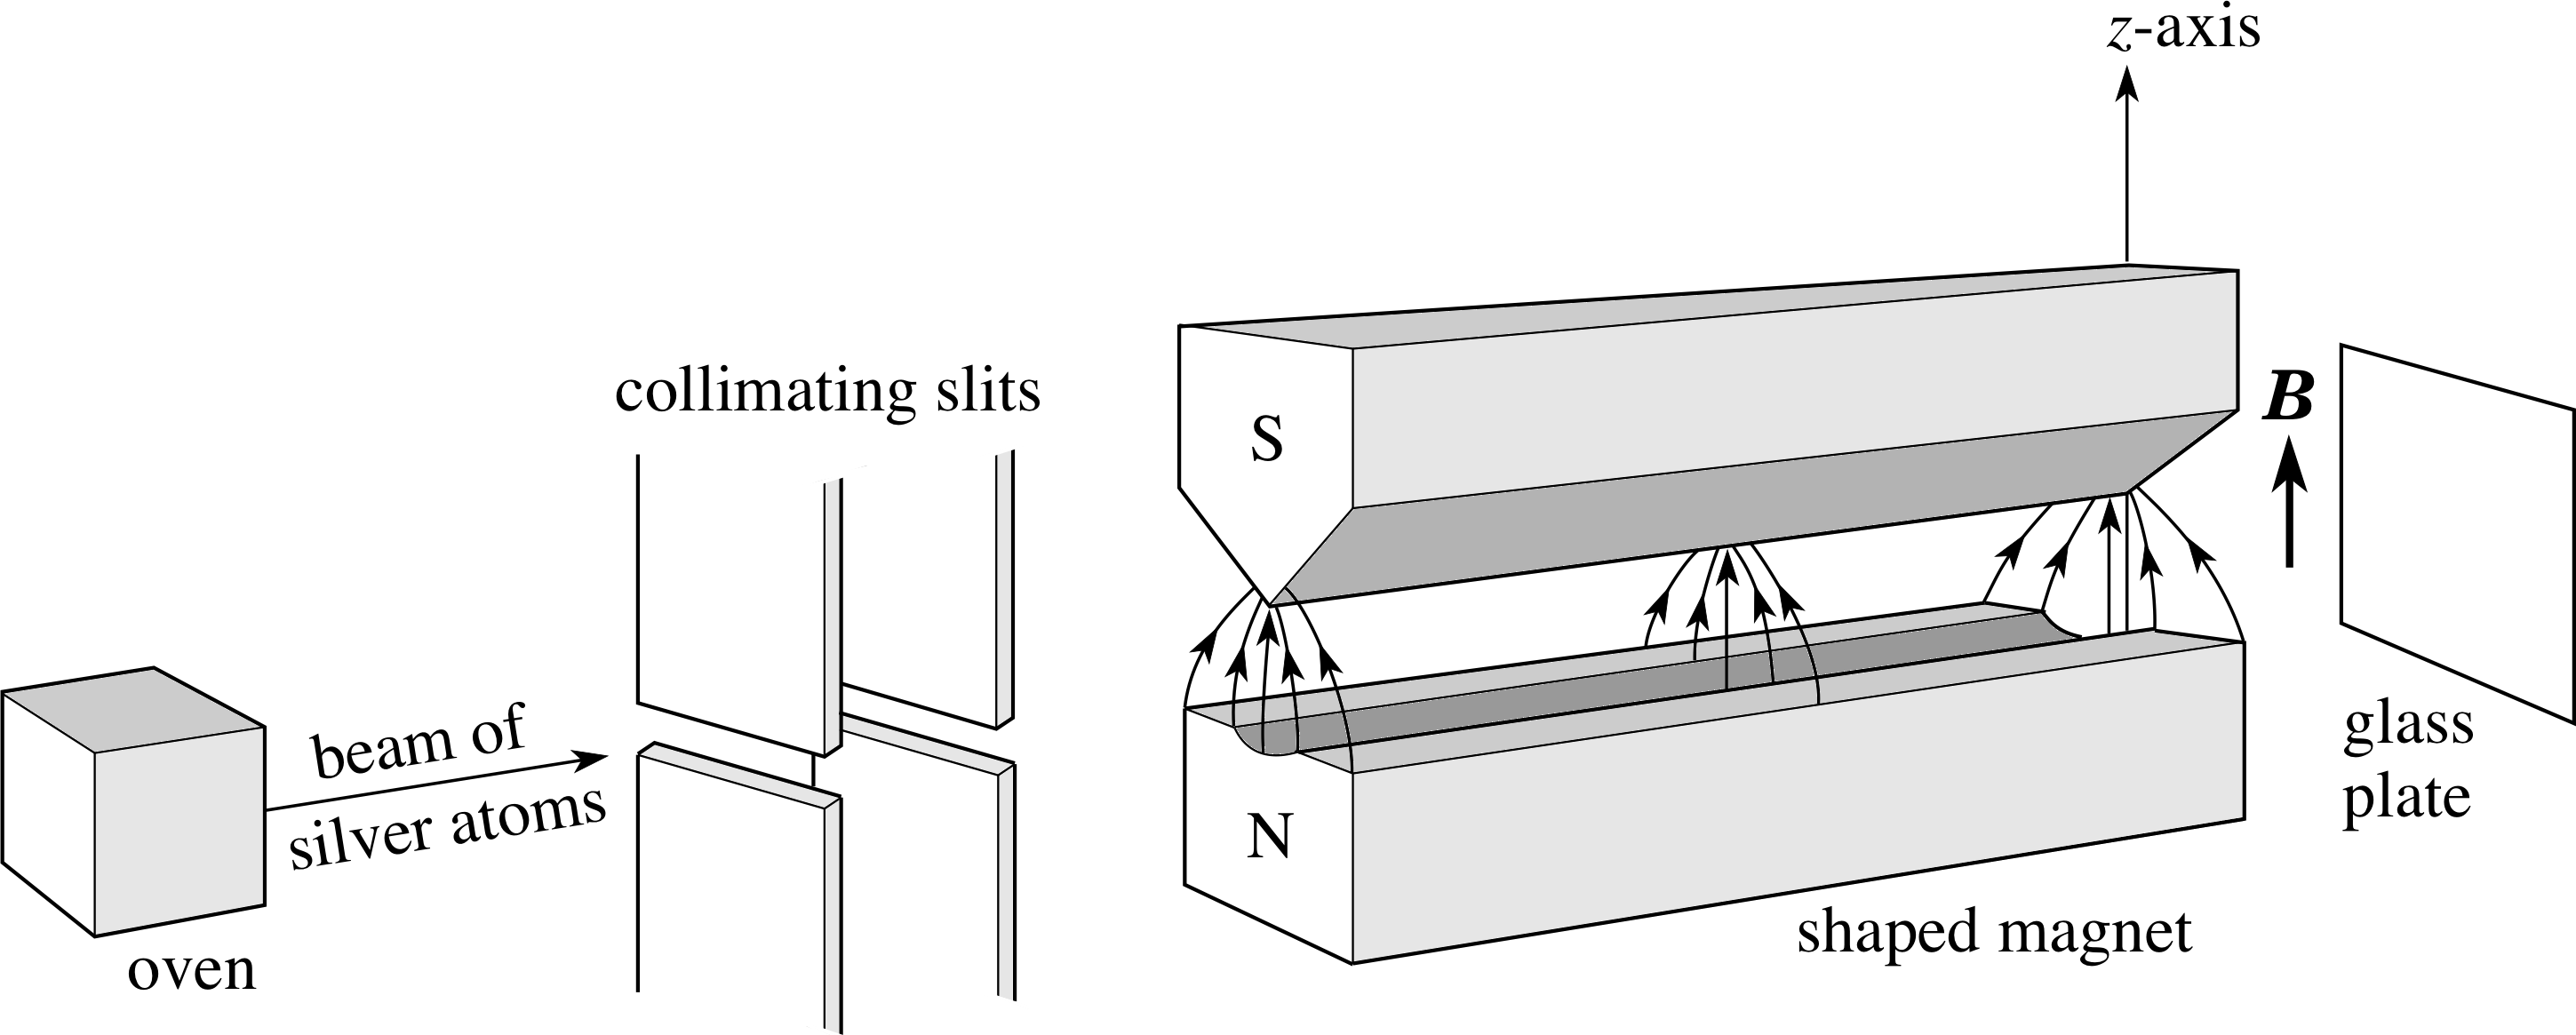
\includegraphics[width=11cm]{Spin/SGexperiment.png}
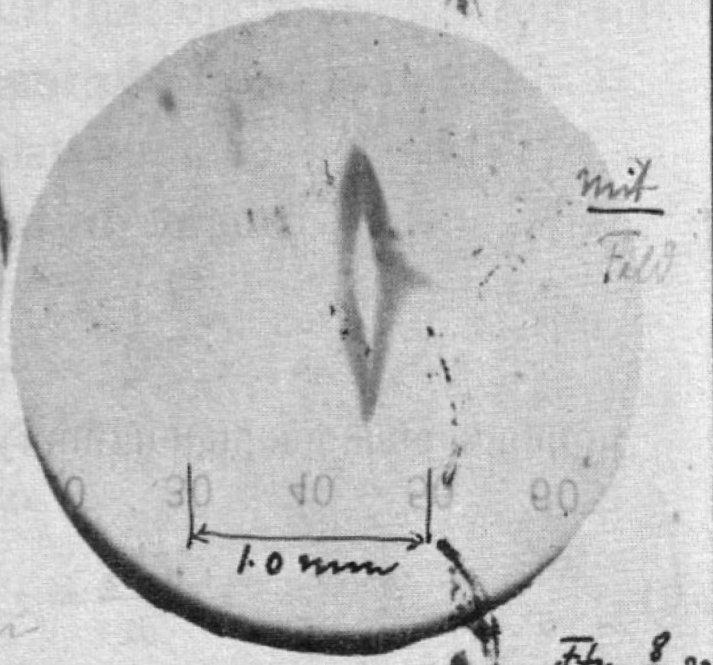
\includegraphics[width=8cm]{Spin/splitting.jpg}
\caption{上:斯特恩-盖拉赫实验装置图。下:最终条纹分裂只有0.2毫米,但很清晰。}
%\label{default}
\end{center}
\end{figure}


积累在靶上的银原子很少,盖拉赫什么都没看到,他把靶板递给斯特恩,这时他们看到银原子积累的痕迹逐渐显现。很神奇,他们把这归结为银的硫化,因为斯特恩当时的薪水很低,他在实验室里抽劣质的雪茄,他们分析可能是劣质雪茄里的硫太多了,使银硫化,而硫化银是黑色的,很容易被看到。

尽管如此,斯特恩和盖拉赫仍然无法得到稳定的图样,他们的结果在证实和否定“空间取向量子化”之间摇摆。同事们也质疑他们的实验,比如德拜就认为“空间取向量子化”根本就不可能被观察到\footnote{“But surely you don’t believe that the (spatial) orientation of atoms is something physically real; that is (only) a timetable for the electrons.”  摘自:“Stern and Gerlach: How a Bad Cigar Helped Reorient Atomic Physics”,Physics Today 56, December 2003, \url{http://zimp.zju.edu.cn/~xinwan/qm2/note/PhysToday_Friedrich03.pdf} }。

斯特恩和盖拉赫都是挺固执的人,面对质疑盖拉赫说:“在这个世界上没有不值得试的事情。”(No experiment is so dumb, that it should not be tried.)

除此之外,他们还碰到很严峻的财务危机,当时德国正处在一战后的困苦中,玻恩竭尽一切办法为斯特恩-盖拉赫实验筹款。他利用公众对相对论的兴趣在学校最大的演讲厅内为爱因斯坦办系列公共演讲,并对参加的听众收取门票。但通货膨胀太厉害了,靠这笔钱也就支持了几个月。最后还是多亏了美国的银行家Goldman(金人)\footnote{Goldman是著名投行Goldman Sachs(高盛)的创始人,他虽然是犹太人但对德国比较友好,1930年代初起移居德国。1936年,在大屠杀发生的前夜,Goldman狼狈逃出德国,保住性命,但其在德财产皆被纳粹没收。}出手寄了几百美元给玻恩。于是,实验继续。

尽管如此,实验进展得仍不如意。1922年,斯特恩去罗斯托克做教授,他和盖拉赫在哥廷根碰头决定放弃实验。但一次铁路罢工改变了这个实验的命运,当时盖拉赫正坐着火车在回法兰克福的途中,因为罢工他在火车上又把实验的种种细节回顾了一遍,他想到了如何改进准直的新主意,回到法兰克福后他继续实验,这一次他获得了非常清晰的分裂条纹。进一步的计算表明,条纹的分裂确实对应$\pm 1$个玻尔磁子($\mu_B $)磁矩的区别,误差在10\%左右。

1922年2月13日,盖拉赫给玻尔寄出一张明信片,背后附有实验结果的照片。明信片上说:“尊敬的玻尔先生:附上我们……所得方向量子化的实验证据。我们祝贺您的理论得到证实。”

表面看这是对玻尔-索末菲理论的直接证实,但其实只是巧合。求解氢原子的薛定谔方程,我们可以得到三个量子数:

\begin{quotation}
主量子数:$n$,$n = 1, 2, ...$

角量子数:$l$,$l = 0, 1, 2, ... n-1$

磁量子数:$m$,$m= 0, \pm 1, \pm 2, \pm l$
\end{quotation}

氢原子的基态,对应$n=1$,$l = 0$,$m = 0$,换句话说氢原子的基态应该是没有角动量的,也没有磁矩。当然斯特恩-盖拉赫实验里用的是银原子,银原子正好只剩一个5s电子在最外层,其他电子在内层,其磁矩都相互抵消掉了。对5s电子而言,$n =5$,$l = 0$,$m = 0$,也没有角动量和磁矩。

那么斯特恩-盖拉赫实验应如何解释呢?实际上它是表明电子具有新角动量——自旋角动量$S$的实验证据。自旋(spin)这个名称来自与经典图像的类别,但这个对比又是不成立的!换句话说这个名字取错了,但名字无非是个指称,物理学家似乎不太在乎这个名字会给门外汉带来误导,他们只是强调自旋是电子(或粒子)的内禀性质,和空间位置($x, y, z$)无关,既然和空间位置无关,我们也就无法把自旋想象成一种在三维空间里发生的自己围绕自己的转动了。

仿照玻恩的句式,我们可以这么说:

\begin{quote}
自旋只是个符号,你要是做字面理解那你可就太Naive了。
\end{quote}

\subsubsection{连续的斯特恩-盖拉赫实验 }

自旋不是真实的,但无论如何斯特恩-盖拉赫实验是真实的。我们可以忘掉玻尔-索末菲理论,继续挖掘这个实验的内涵。

我们把具有$z$方向上的非均匀磁场的斯特恩-盖拉赫装置记做$SGz$,银原子通过$SGz$后将在$z$方向上分裂为两束。分别对应磁矩为$\pm \mu_B$,磁矩是在$z$方向上的,我们称$- \mu_B$的那束为$s_z = \frac{1}{2}\hbar$,$\mu_B$的那束为$s_z = - \frac{1}{2}\hbar$(假设自旋的朗德因子是2,$g_S = 2$,负号很讨厌,这是因为电子带的是负电)。

非均匀磁场的取向是任意的,如果我们设法使银原子通过一个$x$方向非均匀的磁场,即通过SGx,我们会观察到银原子在$x$方向上的分裂,分裂成对称的两束,对应$x$方向上的磁矩$\pm \mu_B$,$- \mu_B $对应的那束是$s_x = \frac{1}{2} \hbar$,$\mu_B $对应的那束是$s_x = - \frac{1}{2} \hbar$。

类似地,我们让银原子通过$y$方向上的非均匀磁场$SGy$,我们会观察到银原子在$y$方向的分裂,也是对称的两束,我们称$- \mu_B$对应的那束是$s_y = \frac{1}{2} \hbar$,$\mu_B$对应的那束是$s_y = - \frac{1}{2} \hbar$。

\begin{figure}[htbp]
\begin{center}
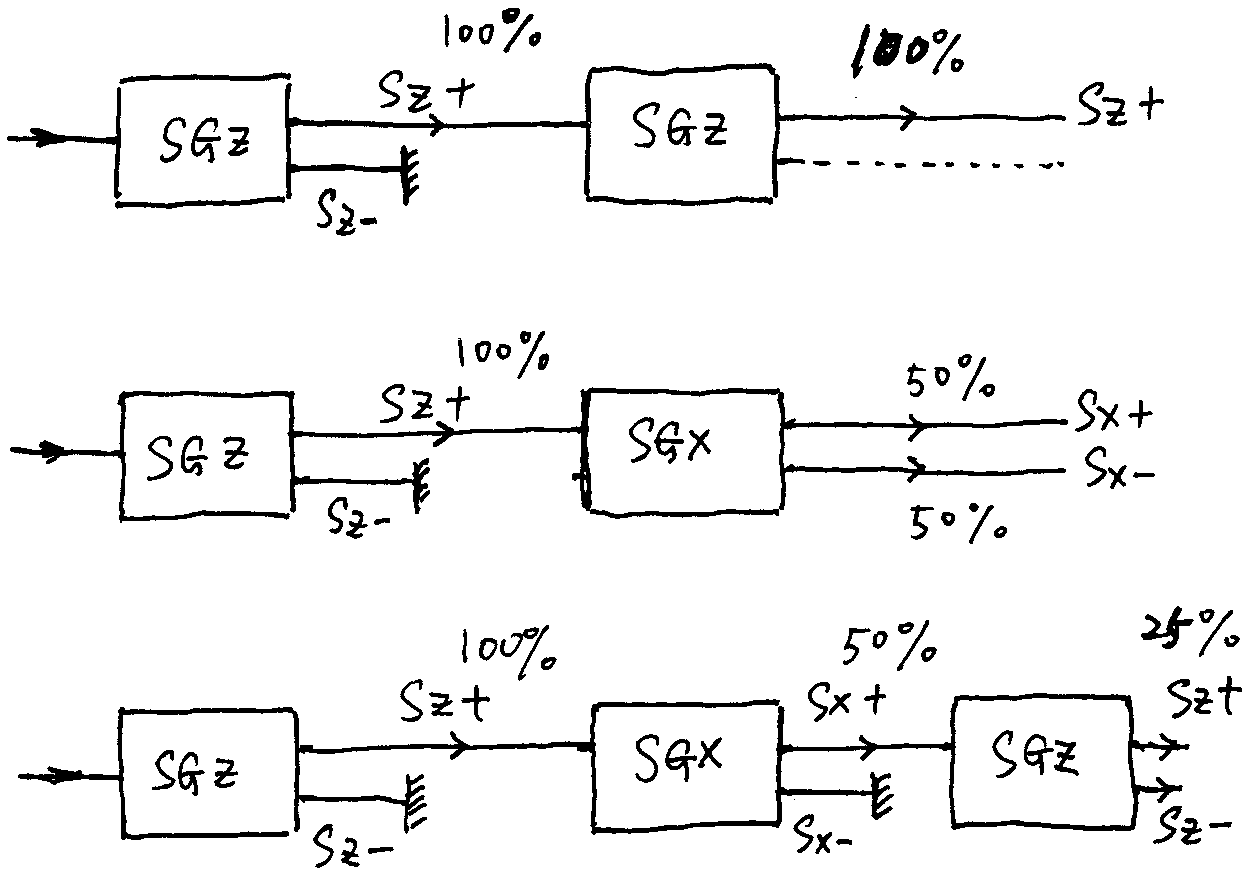
\includegraphics[width=10cm]{Spin/sequentialSGs.png}
\caption{连续的斯特恩-盖拉赫实验。}
%\label{default}
\end{center}
\end{figure}

现在我们使这些实验组合起来,比如:

先让银原子通过SGz,银原子分成对称的两束,我们用隔板挡住$s_z = -\frac{1}{2} \hbar$的那束,只让$s_z = \frac{1}{2} \hbar$的那一束出射,这个动作就是一个选择或过滤的动作。好比我们在一个篮子里放了一堆水果,有香蕉也有苹果,我们现在做一个选择,丢掉香蕉,把苹果留下来。

我们把这种专门选择$s_z = \frac{1}{2}\hbar$的斯特恩-盖拉赫装置记为SGz+,类似地还有SGz-,专门选择$s_z = - \frac{1}{2}\hbar$的银原子。类似地我们还可以定义SGx+,SGx-,SGy+和SGy-。

现在我们来做这样的组合实验:

\begin{equation*}
Ag \to SGz+ \to SGz+ \to ?
\end{equation*}

我们现在使用狄拉克的记号,把$s_z = \frac{1}{2}\hbar$的银原子用记号$\left| z+ \right\rangle$表示。我们用$\left| { ... } \right\rangle$表示量子力学的一个态,括号里面放上可以描述这个态的参数,现在就是z+,和银原子束如何在$z$方向上发生偏转有关。

让银原子束先通过SGz+,即把$\left| z+ \right\rangle$的态选择出来,然后再通过一次SGz+,还是选择$\left| z+ \right\rangle$,最后出射的还是$\left| z+ \right\rangle$。

现在考虑组合:

\begin{equation*}
Ag \to SGz+ \to SGz- \to ?
\end{equation*}

这个组合的作用是先选择$\left| z+ \right\rangle$,再试图从$\left| z+ \right\rangle$中选择$\left| z- \right\rangle$,实验表明最终没有任何银原子出来。这说明:$\left| z+ \right\rangle$和$\left| z- \right\rangle$是两个不相容的态,$\left| z+ \right\rangle$里面完全没有$\left| z- \right\rangle$,$\left| z- \right\rangle$里面完全没有$\left| z+ \right\rangle$。

这就好像是两个互相垂直的矢量$A, B$,A向B投影,或B向A投影都是0,我们可以说A里面完全没有B的成分,相反B里面也完全没有A的成分。

同时把任意的态$\left| \alpha \right\rangle$分解为$\left| z+ \right\rangle$和$\left| z- \right\rangle$的线性组合又是完备的,因为我们使银原子通过SGz时只得到了对称的两束,换句话说在这个标准下对银原子分类只能得到两类。

~

%需要提醒的是,以上陈述都是对实验的陈述,虽然我们有时会用推测式的语气。

下面我们在SGz+和SGz-之间插入一个SGx+:

\begin{equation*}
Ag \to SGz+ \to SGx+ \to SGz- \to ?
\end{equation*}

$x$方向上的非均匀磁场意味着变换了筛选法则。当然我们还可以推测,比如我们把$SGz \pm$想象为对水果种类的筛选,而$SGx \pm$想象为对水果颜色的筛选,那么我们有可能从“红苹果”中找出“香蕉”吗?在这种推测下,我们会认为没有银原子束出射。但最终结果只能实验说了算,实验表明有$\left| z- \right\rangle$态的银原子出来。

类似地,我们还可以做这样的实验:

\begin{center}

$Ag \to SGz+ \to SGx - \to SGz- \to ?$

$Ag \to SGz+ \to SGy + \to SGz- \to ?$

$Ag \to SGz+ \to SGy - \to SGz- \to ?$

$Ag \to SGx+ \to SGy - \to SGx- \to ?$

……

\end{center}

它们都会有银原子出来。

我们管这样的实验叫“连续的斯特恩-盖拉赫实验”(sequential Stern-Gerlach experiment)。

~

现在的问题是如何解释实验。

如果我们认为$\left| z+, x+ \right\rangle$这样的态存在的话,即存在一个对自旋态(我们从现在开始不说银原子了)的陈述,我们可以同时说$s_z = \frac{1}{2}\hbar$而且$s_x = \frac{1}{2}\hbar$,那么我们就没法从$\left| z+, x+ \right\rangle$中筛选出$\left| z- \right\rangle$。

%%

为了理解连续的“斯特恩-盖拉赫实验”,我们只有求助于比喻,即用我们熟悉的现象来类比,而建立比喻并不需要两种现象很像或……,所谓比喻是可以任意建立的,比如这里我们可以建立一个“颜色-形状”比喻来理解连续的“斯特恩-盖拉赫实验”。

假想在黑箱里有一堆小物件,我们应如何对其分类呢?比如颜色是一个分类的标准,形状是另一个分类的标准,颜色和形状是完全不相干的描述物件性质的两个标准。

我们说一个小物件是白色的;或是黑色的;白色和黑色是两种互相排斥的陈述,只要是白色的就不能是黑色的,相反只要是黑色的就不能是白色的。

我们也说一个小物件是个立方体,或说它是个球体。球体和立方体也是互相排斥的,我们没法说它既是球体又是立方体。

假设在我们的世界里,这个小物件不是立方体就是球体,但不能既是立方体又是球体。类似的我们说在我们的世界里,这个小物体不是白色的就是黑色的,但不能既是白色的又是黑色的。

形状是我们对物件的陈述,颜色也是我们对物件的陈述。现在我们的问题是:我们能够同时使用颜色和形状来陈述一个物件吗?

在经典世界里,或在我们的日常经验中,当然可以,香蕉是黄色的,同时它也是弯曲的棒棒形,形状和颜色是我们一眼看去可以直观的。

但在量子世界里,这种陈述是被禁止的!看清楚了物件的颜色,物件就完全没有形状;同样看清楚了物件的形状,那它就没有颜色\footnote{使用苹果、香蕉的语言:

设想我们先筛选出苹果,然后换个筛选标准,对苹果按颜色筛选,筛选出所有“红色的苹果”,注意!问题就在这里,一旦你说出了“红色的苹果”这一陈述,我们就没法从“红色的苹果”中筛选出香蕉了。

正确的陈述是:

我们首先筛选出苹果,然后换个筛选标准,对苹果按颜色筛选,但这两个标准是相克的,我们一旦知道了颜色,我们就完全丧失形状的信息,现在我们只知道是红色的,但完全不知道到底是苹果和香蕉,最后我们是对红色的水果筛选出香蕉。}。

这非常反直觉。但需记住,这种叙事是基于比喻建立的,如果我们换一个比喻的话,比如光的偏振现象,我们就会觉得一切都会来的很舒服。(对相同事件,切换视角,任意武断地使用比喻(图像)进行叙事是发现的门径。)

\subsubsection{与光偏振现象的类比}

我们现在来建立对连续斯特恩-盖拉赫实验的数学描述,考虑:

\begin{equation*}
Ag \to SGz+ \to SGx+ \to SGz- \to ?
\end{equation*}

假设银原子从SGz+出来的比例是100\%,通过SGx+后就只剩下50\%,然后通过SGz-还剩25\%银原子。

\begin{figure}[htbp]
\begin{center}
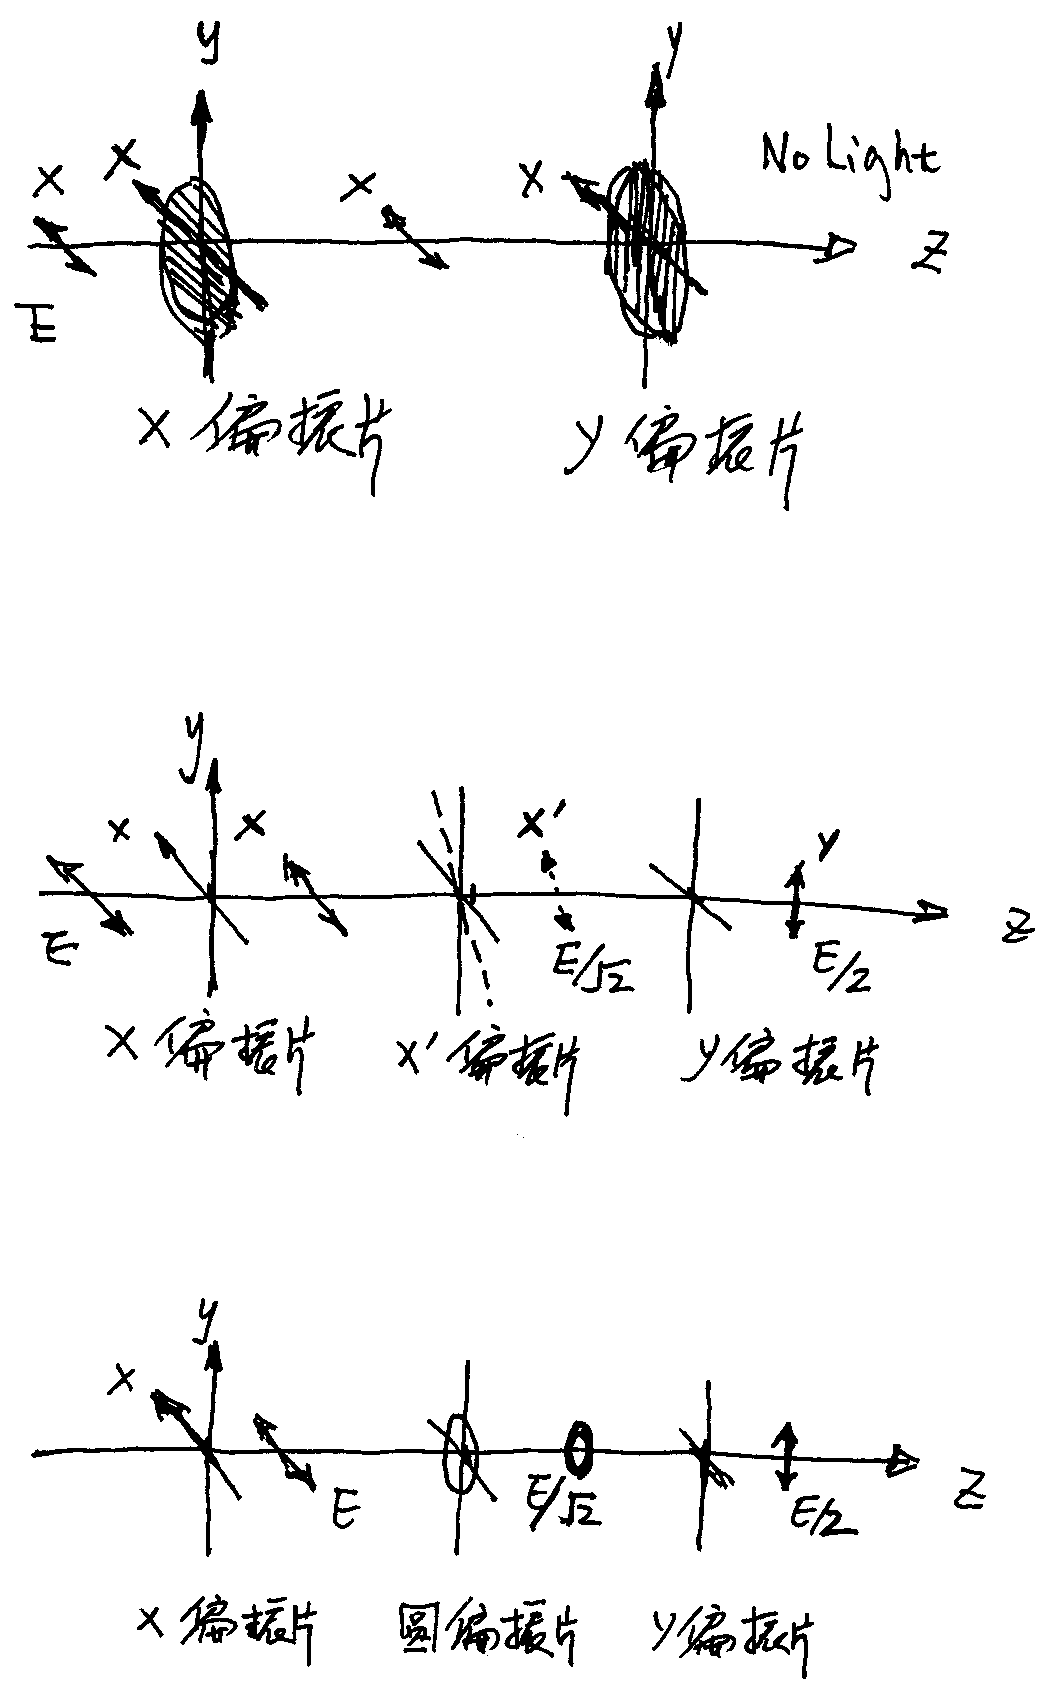
\includegraphics[width=10cm]{Spin/sequentiallightpolarization.png}
\caption{连续的偏振光实验}
%\label{default}
\end{center}
\end{figure}

我们可以通过与光偏振现象的类比来建立自旋的理论。光有线偏振光,还有圆偏振光。

比如我们使偏振片的偏振方向与x轴平行,它的作用就是使电矢量垂直于x轴的光统统被吸收,而电矢量平行于x轴的光全部通过。这样我们就得到一个x偏振的光,这也是筛选。

对一束x偏振的光而言,没有任何y偏振的成分,相反亦然,这可以类比态$\left|z+ \right\rangle $和$\left| z- \right\rangle$,它们都是互相排斥的分类标准。
 
~

现在使偏振片旋转$45^o$,我们称之为x'偏振片,它筛选出x'方向的偏振光,继续旋转$90^o$得到y'偏振片,筛选出y'偏振光,x'和y'是垂直的,因此x'偏振光中不会有任何y'的成分,反之亦然。

并且如果我们让一束光先通过x偏振片再通过x'偏振片,最后通过y偏振片的话,我们会看到出射光,而且百分比和刚才连续的斯特恩-盖拉赫实验的实验结果是一致的。

因此,我们就可以用x'偏振光来类比态$\left|x+ \right\rangle$,y'偏振光来类比$\left|x- \right\rangle$。

但我们还有态$\left| y+ \right\rangle$和$\left| y- \right\rangle$,它们应和什么样的偏振光来类比呢?

我们还有圆偏振光,R右旋光和L左旋光是互相排斥的分类标准,正好可以对应态$\left| y+ \right\rangle$和$\left| y- \right\rangle$。

现在我们的问题就转换为如何描述偏振光了,假设光沿$z$方向传播,光是横波,电矢量只能在$x-y$平面上振动,因此我们用$x-y$平面上的一个矢量来表示:

\begin{figure}[htbp]
\begin{center}
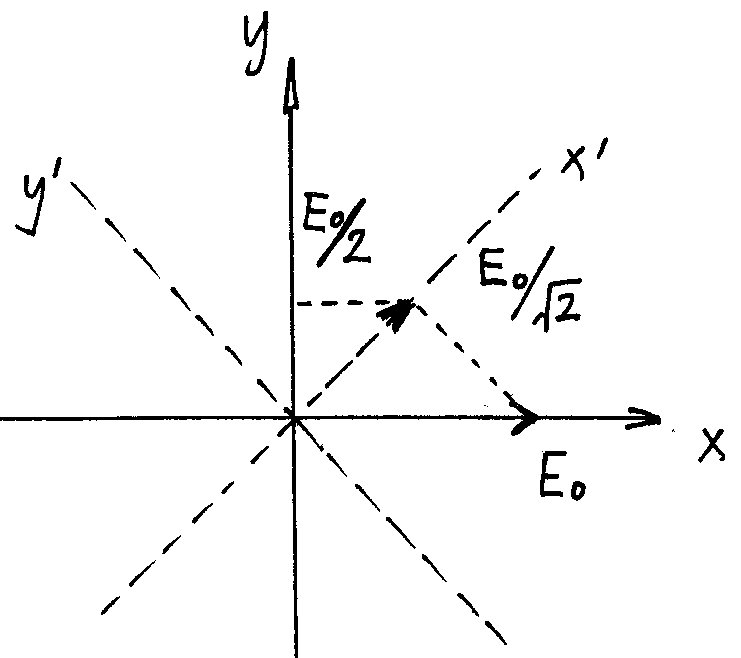
\includegraphics[width=8cm]{Spin/E0_projection.png}
\caption{振幅为$E_0$的x线偏振光先向x'方向投影,振幅变为$\frac{E_0}{\sqrt{2}}$,最后向y方向投影,振幅变为$\frac{E_0 }{2}$。光强正比于振幅的平方,因此光强的比为:100\% : 50\% : 25\%。}
%\label{default}
\end{center}
\end{figure}

$x-y$平面里的任意矢量可以表示为一个二维列向量,如矢量:

\begin{equation*}
V = 1 \cdot e_x + 0 \cdot e_y  \dot =\left( \begin{array}{ccc} 1 \\ 0 \end{array} \right) 
\end{equation*}

我们可以用一个二维的列向量来描述任意一束偏振光,但为了描述圆偏振光,列向量中必须出现纯虚数$i$,换句话说我们是用一个复系数的二维列向量来描述沿$z$方向传播的光的偏振态的。

%%

\begin{enumerate}
\item 

沿$z$轴传播的x线偏振光可表示为:

\begin{equation}
E^{x} = E_0 e_x \cos (k z - \omega t) 
\end{equation}

沿$z$轴传播的y线偏振光可表示为:

\begin{equation}
E^{y} = E_0 e_y \cos (k z - \omega t) 
\end{equation}

这里$e_x, e_y$分别是$x$轴和$y$轴上的单位向量。我们一般把它们写为列向量的形式,第一行对应$e_x$分量,第二行对应$e_y$分量。

\begin{eqnarray}
E^{x} & = & \left( \begin{array}{ccc} 1 \\ 0  \end{array} \right)  E_0 \cos (kz - \omega t )  \\
E^{y} & = & \left( \begin{array}{ccc} 0 \\ 1  \end{array} \right)  E_0 \cos (kz - \omega t )
\end{eqnarray}

再把它们改写为复数的形式。

\begin{eqnarray}
E^{x} & = & \Re \left( \begin{array}{ccc} 1 \\ 0  \end{array} \right)  E_0 e^{i ( kz - \omega t  )}  \\
E^{y} & = & \Re \left( \begin{array}{ccc} 0 \\ 1  \end{array} \right)  E_0 e^{i ( kz - \omega t  ) }  
\end{eqnarray}

\item

沿$z$轴传播的x'和y'线偏振光可表示为:

\begin{eqnarray}
E^{x'} & = & \Re \left( \begin{array}{ccc} 1 \\ 1  \end{array} \right)  \frac{ E_0 }{ \sqrt{2} }   e^{i ( kz - \omega t  )}  \\
E^{y'} & = & \Re \left( \begin{array}{ccc} -1 \\ 1  \end{array} \right)  \frac{E_0}{ \sqrt{2} }  e^{i ( kz - \omega t  ) }  
\end{eqnarray}

\item

沿$z$轴传播的右旋R圆偏振光和左旋L圆偏振光可表示为:

\begin{eqnarray}
E^{R} & = & \Re \left( \begin{array}{ccc} 1 \\ i  \end{array} \right)  \frac{ E_0 }{ \sqrt{2} }   e^{i ( kz - \omega t  )}  \\
E^{L} & = & \Re \left( \begin{array}{ccc} 1 \\  -i  \end{array} \right)  \frac{E_0}{ \sqrt{2} }  e^{i ( kz - \omega t  ) }  
\end{eqnarray}

\end{enumerate}

由于我们把自旋的态类比为光的偏振态,因此我们可以尝试把自旋的态表示为一个复系数二维向量空间中的一个向量。

\begin{enumerate}
\item 

我们分别用x线偏振光和y线偏振光来表示$\left| z+ \right\rangle$和$\left| z+ \right\rangle$。即尝试性地把$\left| z+ \right\rangle$表示为列向量$\left( \begin{array}{ccc} 1 \\ 0   \end{array} \right)$,把$\left| z- \right\rangle$表示为列向量$\left( \begin{array}{ccc} 0 \\ 1 \end{array} \right)$。即:

\begin{eqnarray}
\left| z+ \right\rangle & \dot = & \left( \begin{array}{ccc} 1 \\ 0   \end{array} \right) \\
\left| z- \right\rangle & \dot = & \left( \begin{array}{ccc} 0 \\ 1 \end{array} \right)
\end{eqnarray}

这里$\dot =$读作“表示为”,以示与“等于”的区分\footnote{等于只用于同类间的关系,而“表示为”或比喻则可用不同类的现象互为引证。}。

\item

态$\left| x \pm \right\rangle$可表示为:

\begin{eqnarray}
\left| x + \right\rangle & \dot = & \frac{1}{\sqrt{2}}  \left( \begin{array}{ccc}  1 \\ 1 \end{array}  \right)  \\
\left| x - \right\rangle  & \dot =  & \frac{1}{\sqrt{2}}  \left( \begin{array}{ccc}  -1 \\ 1 \end{array} \right)
\end{eqnarray}

\item

态$\left| y \pm \right\rangle$可表示为:

\begin{eqnarray}
\left| y + \right\rangle & \dot = & \frac{1}{\sqrt{2}}  \left( \begin{array}{ccc}  1 \\ i  \end{array} \right)  \\
\left| y - \right\rangle  & \dot =  & \frac{1}{\sqrt{2}}  \left( \begin{array}{ccc}  1 \\ -i \end{array} \right)
\end{eqnarray}

\end{enumerate}



\subsection*{练习}

\begin{enumerate}
\item 

斯特恩-盖拉赫实验,银原子束从温度为600K的炉子跑出来,经过准直装置后,通过一个0.1米长的非均匀磁场,磁场的梯度是$\frac{\partial B_z}{\partial z} = 10^3$特斯拉/米。银原子从非均匀磁场跑出来后又继续“飞”了1米,求最终银原子在靶上的分裂宽度是多少。(假设银原子的平均速度为$v$,它的平均动能是$\frac{M v^2}{2} = \frac{3 k_B T}{2}$,这里$M$是银原子的质量,$k_B$是玻尔兹曼因子。)

\end{enumerate}